\documentclass{beamer}
\usepackage[utf8]{inputenc}
\usepackage[T1]{fontenc}
\usepackage[french]{babel}
\usepackage{amsmath,amssymb,amsfonts}
\usepackage{graphicx}
\usepackage{booktabs}
\usepackage{listings}

\usetheme{Madrid}
\usecolortheme{default}

\title[Adam vs L-BFGS]{Optimisation Numérique : Adam vs L-BFGS}
\author[KABLAM]{KABLAM Edjabrou Ulrich Blanchard}
\institute[AMA]{Académie des Mathématiques Appliquées}
\date{\today}

\lstset{
    basicstyle=\ttfamily\tiny,
    breaklines=true,
    frame=single,
    language=Python,
    showstringspaces=false
}

\begin{document}

\begin{frame}
    \titlepage
\end{frame}

\begin{frame}{Table des matières}
    \tableofcontents
\end{frame}

% =========================================================================
\section{Introduction et mise en contexte}
% =========================================================================

\begin{frame}{1. Introduction : Historique et Évolution}
    \begin{block}{Contexte des méthodes d'optimisation}
        L'optimisation numérique est essentielle en sciences et en ingénierie pour minimiser des fonctions de coût $f(\theta)$ par rapport à des paramètres $\theta \in \mathbb{R}^n$ \cite{kingma2014adam}.
    \end{block}
    
    \begin{itemize}
        \item \textbf{Années 1950-1970 (L'ère classique) :} Naissance de la descente de gradient, puis des méthodes quasi-Newton (Broyden 1965, DFP 1959, et BFGS en 1970 découvert indépendamment par Broyden, Fletcher, Goldfarb et Shanno) \cite{gramfort_quasi_newton}.
        \item \textbf{Années 2011-2015 (L'ère adaptative pour le Big Data) :} Apparition d'AdaGrad (2011), RMSProp (2012) et enfin \textbf{Adam} (Adaptive Moment Estimation) par Kingma \& Ba en 2015 à ICLR \cite{kingma2014adam}.
    \end{itemize}
\end{frame}

\begin{frame}{Définitions Fondamentales}
    \begin{definition}[Complexité Algorithmique]
        La complexité algorithmique mesure la façon dont les ressources (temps d'exécution ou espace mémoire) évoluent en fonction de la taille $n$ du problème (nombre de paramètres) en utilisant la notation Grand O ($O$).
    \end{definition}

    \begin{definition}[Méthodes de Premier et Second Ordre]
        \begin{itemize}
            \item \textbf{Premier ordre :} Utilisent uniquement le gradient $\nabla f(\theta)$ (la pente) \cite{kingma2014adam}.
            \item \textbf{Second ordre :} Utilisent ou approximent la matrice Hessienne $\nabla^2 f(\theta)$ (la courbure) \cite{gramfort_quasi_newton}.
        \end{itemize}
    \end{definition}
\end{frame}

% =========================================================================
\section{Concepts mathématiques et algorithmes}
% =========================================================================
\begin{frame}{La Méthode de Descente de Gradient}
    \begin{block}{Équation de mise à jour}
        La méthode de descente de gradient cherche à minimiser une fonction objectif en suivant la direction de la plus forte pente (le gradient négatif) \cite{synapsara_video} via l'itération :
        \begin{equation}
            x_{k+1} = x_k - \alpha \nabla f(x_k)
        \end{equation}
        où $\alpha > 0$ représente le pas d'apprentissage (\emph{learning rate}) \cite{synapsara_video}.
    \end{block}
    \begin{itemize}
        \item \textbf{Convergence :} Linéaire et souvent lente, en particulier dans les vallées étroites (problèmes mal conditionnés) où l'algorithme zoome en zigzaguant \cite{synapsara_video}.
        \item \textbf{Complexité :} Très efficace en mémoire avec une complexité spatiale en $O(n)$, ce qui la rend hautement scalable pour le Deep Learning comparativement aux méthodes du second ordre \cite{synapsara_video}.
    \end{itemize}
\end{frame}

\begin{frame}{1. La Méthode de Newton}
    \begin{block}{Équation de mise à jour}
        La méthode de Newton cherche les points stationnaires ($\nabla f(x) = 0$) via l'itération \cite{gramfort_quasi_newton} :
        \begin{equation}
            x_{k+1} = x_k - \left(\nabla^2 f(x_k)\right)^{-1} \nabla f(x_k)
        \end{equation}
    \end{block}
    \begin{itemize}
        \item \textbf{Convergence :} Quadratique locale \cite{gramfort_quasi_newton}.
        \item \textbf{Complexité :} Stocker et inverser la Hessienne $n \times n$ coûte $O(n^2)$ en mémoire et $O(n^3)$ en calcul, ce qui est explosif pour le Deep Learning \cite{synapsara_video}.
    \end{itemize}
\end{frame}

\begin{frame}{2. Les Méthodes Quasi-Newton : BFGS}
    \begin{block}{Approximation de la Hessienne inverse}
        Au lieu de calculer la Hessienne, BFGS l'approxime par une matrice $B_k$ mise à jour par une correction de rang 2 \cite{gramfort_quasi_newton} :
        \begin{equation}
            H_{k+1} = H_k + \frac{y_k y_k^T}{y_k^T s_k} - \frac{H_k s_k s_k^T H_k}{s_k^T H_k s_k}
        \end{equation}
        avec $s_k = x_{k+1} - x_k$ et $y_k = g_{k+1} - g_k$.
    \end{block}
    \begin{itemize}
        \item \textbf{Limite mémoire :} Stockage de la matrice en $O(n^2)$, soit 8 To pour 1 million de paramètres \cite{synapsara_video}.
    \end{itemize}
\end{frame}

\begin{frame}{3. L-BFGS (Limited-memory BFGS)}
    \begin{block}{Algorithme 3 : Direction finding (L-BFGS)}
        L-BFGS contourne le problème en ne stockant que les $3<m<20$ derniers vecteurs $(s_i, y_i)$ (où $m \ll n$) et utilise la récursion à deux boucles (\emph{two-loop recursion}) \cite{gramfort_quasi_newton} :
        \begin{equation}
            \text{Complexité Mémoire :} \quad O(m \cdot n)
        \end{equation}
    \end{block}
    \begin{itemize}
        \item Pour $n = 10^6$ et $m = 10$, on passe de 8 To à seulement 80 Mo de mémoire \cite{synapsara_video}.
    \end{itemize}
\end{frame}

\begin{frame}{4. L'Algorithme Adam : Origine et Objectif}
    \begin{definition}[Signification d'ADAM]
        \textbf{ADAM} signifie \textbf{ADA}ptive \textbf{M}oment estimation (Estimation de Moments Adaptatifs) \cite{kingma2014adam}.
    \end{definition}

    \begin{block}{Par qui et pourquoi a-t-il été créé ? (Kingma \& Ba, 2015)}
        Créé par Diederik Kingma et Jimmy Ba en 2015 \cite{kingma2014adam}, Adam a été conçu pour \textbf{combiner les meilleurs avantages de deux mondes} :
        \begin{itemize}
            \item \textbf{AdaGrad :} pour son efficacité redoutable sur les gradients éparses (\emph{sparse gradients}) \cite{kingma2014adam}.
            \item \textbf{RMSProp :} pour sa robustesse dans les contextes en ligne (\emph{online}) et non-stationnaires \cite{kingma2014adam}.
        \end{itemize}
    \end{block}

    \begin{itemize}
        \item \textbf{Qu'est-ce que ça fait ?} Il calcule des taux d'apprentissage adaptatifs individuels pour chaque paramètre du modèle à partir des estimations des premier et second moments des gradients \cite{kingma2014adam}.
    \end{itemize}
\end{frame}

\begin{frame}{4. L'Algorithme Adam (Kingma \& Ba, 2015)}
    \begin{block}{Algorithme 1 : Mises à jour des moments}
        Adam combine momentum et taux adaptatifs \cite{kingma2014adam} :
        \begin{align}
            m_t &= \beta_1 m_{t-1} + (1 - \beta_1) g_t \\
            v_t &= \beta_2 v_{t-1} + (1 - \beta_2) g_t^2
        \end{align}
    \end{block}
    \end{frame}
    \begin{frame}
\begin{block}{Correction du biais et mise à jour}
        \begin{equation}
            \hat{m}_t = \frac{m_t}{1 - \beta_1^t}, \quad \hat{v}_t = \frac{v_t}{1 - \beta_2^t}
        \end{equation}
        \begin{equation}
            \theta_{t+1} = \theta_t - \frac{\alpha}{\sqrt{\hat{v}_t} + \epsilon} \hat{m}_t
        \end{equation}
        où \textbf{$\epsilon = 10^{-8}$} est une petite constante de stabilisation ajoutée au dénominateur \cite{kingma2014adam}. 
        \textbf{Pourquoi l'utiliser ?} Elle est indispensable pour \textbf{éviter une division par zéro} au cas où le moment second $\hat{v}_t$ deviendrait nul ou extrêmement proche de zéro, garantissant ainsi la stabilité numérique de l'algorithme \cite{kingma2014adam}.
    \end{block}
\end{frame}

\begin{frame}{Comparaison : L-BFGS vs Adam}
    \begin{table}
        \centering
        \caption{Tableau comparatif des optimiseurs L-BFGS et Adam.}
        \resizebox{\textwidth}{!}{% Ajuste automatiquement la taille à la largeur de la slide
        \begin{tabular}{lll}
            \toprule
            \textbf{Caractéristique} & \textbf{L-BFGS} & \textbf{Adam} \\
            \midrule
            Type & Second ordre \cite{gramfort_quasi_newton} & Premier ordre \cite{kingma2014adam} \\
            Données & Batch / Déterministe \cite{synapsara_video} & Stochastique / Mini-batch \cite{kingma2014adam} \\
            Mémoire & $O(m \cdot n)$ \cite{gramfort_quasi_newton} & $O(n)$ \cite{kingma2014adam} \\
            Usage & Problèmes lisses, modérés \cite{gramfort_quasi_newton} & Deep Learning massif \cite{kingma2014adam} \\
            \bottomrule
        \end{tabular}
        }
    \end{table}
    \vspace{0.2cm}
    \tiny{\textbf{Note :} \textit{Batch / Déterministe} = calcul du gradient sur tout le dataset sans aucun hasard (très précis, mais consomme énormément de mémoire et de temps pour des millions de lignes). 
    
    \textit{Stochastique / Mini-batch} = calcul par petits groupes aléatoires de données (introduit du bruit, mais accélère les mises à jour et évite de saturer le GPU ; le bruit est géré par les moyennes mobiles $m_t$ et $v_t$ d'Adam).}

\end{frame}

\begin{frame}{Comparaison Empirique : Adam vs L-BFGS}
    \begin{figure}
        \centering
        % Remplacer image1.png et image2.png par les noms réels de vos fichiers d'images
        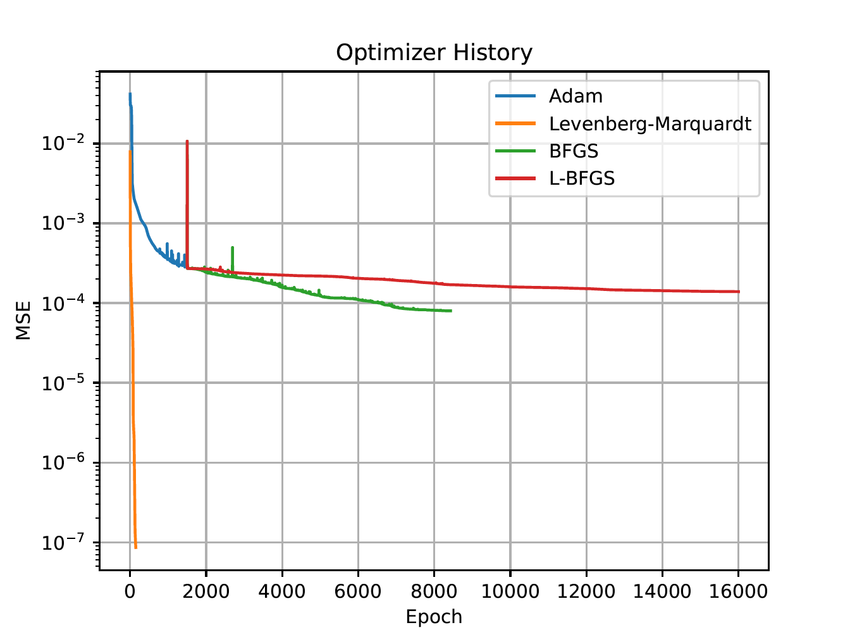
\includegraphics[width=0.45\textwidth]{image1.png}\hfill
        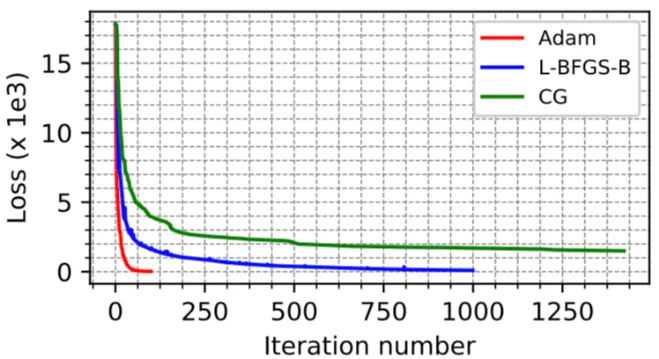
\includegraphics[width=0.45\textwidth]{image2.png}
        \caption{Évolution de la Loss et du MSE comparant Adam et L-BFGS sur des problèmes non-linéaires et réseaux profonds.}
    \end{figure}
    \tiny{
        \textbf{Sources des graphiques :} 
        \begin{itemize}
            \item \textbf{Gauche :} Sun et al., \emph{A deep learning perspective of the forward and inverse problems in exploration geophysics} (2019) \cite{sun2019deep}.
            \item \textbf{Droite :} Etude comparative sur les réseaux de neurones informés par la physique / deep learning (2020) \cite{optimizer_history_2020}.
        \end{itemize}
    }
\end{frame}
\begin{frame}{Analyse Empirique : Adam vs L-BFGS}
    \begin{block}{Contexte des expériences}
        Ces graphiques comparent la vitesse de convergence des optimiseurs (notamment Adam et L-BFGS) sur des architectures de réseaux de neurones complexes et des problèmes d'optimisation non-linéaires \cite{sun2019deep, optimizer_history_2020}. 
    \end{block}

    \begin{itemize}
        \item \textbf{Observations (Graphique de gauche - MSE / Époque) :} Le modèle commence souvent par une phase d'entraînement avec Adam, puis bascule sur des méthodes de second ordre. On remarque la chute spectaculaire et ultra-rapide de l'erreur initiale pour Adam \cite{optimizer_history_2020}.
        \item \textbf{Observations (Graphique de droite - Loss / Itérations) :} Adam (courbe rouge) s'effondre vers une loss minimale en un nombre d'itérations extrêmement faible ($\approx 100$ itérations), surclassant nettement L-BFGS et le gradient conjugué (CG) \cite{sun2019deep}.
        \end{itemize}
        \end{frame}
        \begin{frame}
        \begin{itemize}
        \item \textbf{Lequel est le meilleur et pourquoi ?} 
        \begin{itemize}
            \item \textbf{Adam} est globalement supérieur en phase initiale et pour le Deep Learning massif : ses taux d'adaptativité par paramètre gèrent mieux le bruit stochastique des mini-batchs.
            \item \textbf{L-BFGS} peut offrir une précision chirurgicale en fin d'optimisation sur des problèmes déterministes, mais s'avère beaucoup plus lent à converger au début en raison de l'estimation de sa courbure.
        \end{itemize}
    \end{itemize}
\end{frame}
% =========================================================================
\section{Programmation Python et applications}
% =========================================================================
\begin{frame}[fragile]{Annexe : Implémentation Python From Scratch (1/2)}
    \begin{lstlisting}
import numpy as np
import time
import matplotlib.pyplot as plt

def fonction_cout(theta, X, y):
    m = len(y)
    return (1 / (2 * m)) * np.sum((X @ theta - y) ** 2)

def gradient(theta, X, y):
    m = len(y)
    return (X.T @ (X @ theta - y)) / m

def optimiseur_adam(X, y, theta_init, alpha=0.001, beta1=0.9, beta2=0.999, epsilon=1e-8, n_iter=100):
    theta = theta_init.copy()
    m = np.zeros_like(theta)
    v = np.zeros_like(theta)
    historique_cout = []
    
    for t in range(1, n_iter + 1):
        gt = gradient(theta, X, y)
        m = beta1 * m + (1 - beta1) * gt
        v = beta2 * v + (1 - beta2) * (gt ** 2)
        m_hat = m / (1 - (beta1 ** t))
        v_hat = v / (1 - (beta2 ** t))
        theta = theta - (alpha / (np.sqrt(v_hat) + epsilon)) * m_hat
        historique_cout.append(fonction_cout(theta, X, y))
        
    return theta, historique_cout
    \end{lstlisting}
\end{frame}

\begin{frame}[fragile]{Annexe : Implémentation Python From Scratch (2/2)}
    \begin{lstlisting}
def optimiseur_l_bfgs(X, y, theta_init, m_history=10, n_iter=100):
    theta = theta_init.copy()
    historique_cout = []
    s_list, y_list = [], []
    
    for k in range(n_iter):
        gk = gradient(theta, X, y)
        historique_cout.append(fonction_cout(theta, X, y))
        if k == 0:
            pk = -gk # Premier pas en descente de gradient pure
        else:
            # Algorithme 3 : Recursion a deux boucles (Two-loop recursion)
            q = gk.copy()
            alphas = []
            for s, y_vec in reversed(list(zip(s_list, y_list))):
                rho = 1.0 / (y_vec @ s)
                alpha = rho * (s @ q)
                alphas.append(alpha)
                q -= alpha * y_vec
            
            # Matrice initiale H0 approchee par un scalaire
            gamma = (s_list[-1] @ y_list[-1]) / (y_list[-1] @ y_list[-1])
            r = gamma * q
            
            for (s, y_vec), alpha in zip(zip(s_list, y_list), reversed(alphas)):
                rho = 1.0 / (y_vec @ s)
                beta = rho * (y_vec @ r)
                r += s * (alpha - beta)
            pk = -r
            
        # Pas fixe ou line search simplifiee
        alpha_step = 0.01
        theta_next = theta + alpha_step * pk
        sk = theta_next - theta
        yk_vec = gradient(theta_next, X, y) - gk
        
        # Gestion de la memoire limite m
        s_list.append(sk)
        y_list.append(yk_vec)
        if len(s_list) > m_history:
            s_list.pop(0)
            y_list.pop(0)
        theta = theta_next
    return theta, historique_cout
    \end{lstlisting}
\end{frame}

\begin{frame}[fragile]{Annexe : Benchmark, Mesure de Temps et Tracé}
    \begin{lstlisting}
# --- Generation de donnees de test ---
np.random.seed(42)
X_synth = np.c_[np.ones(500), np.random.rand(500, 5)]
vrai_theta = np.array([2.0, -1.0, 3.5, 0.5, -2.0, 1.0])
y_synth = X_synth @ vrai_theta + np.random.randn(500) * 0.1
theta_0 = np.zeros(6)

# --- Execution et Mesure du Temps pour Adam ---
t_start_adam = time.time()
th_adam, cout_adam = optimiseur_adam(X_synth, y_synth, theta_0, alpha=0.05, n_iter=200)
t_adam = time.time() - t_start_adam

# --- Execution et Mesure du Temps pour L-BFGS ---
t_start_lbfgs = time.time()
th_lbfgs, cout_lbfgs = optimiseur_l_bfgs(X_synth, y_synth, theta_0, m_history=5, n_iter=200)
t_lbfgs = time.time() - t_start_lbfgs

print(f"Temps Adam : {t_adam:.4f}s | Temps L-BFGS : {t_lbfgs:.4f}s")

# --- Trace des graphiques comparatifs ---
plt.figure(figsize=(7, 3.5))
plt.plot(cout_adam, label=f"Adam (Temps: {t_adam:.3f}s)", color="red")
plt.plot(cout_lbfgs, label=f"L-BFGS (Temps: {t_lbfgs:.3f}s)", color="blue")
plt.xlabel("Iterations")
plt.ylabel("Fonction de Cout (MSE)")
plt.legend()
plt.title("Comparaison de Convergence : Adam vs L-BFGS")
plt.grid(True)
plt.show()
    \end{lstlisting}
\end{frame}
\begin{frame}{Résultat Pratique : Benchmark From Scratch (Adam vs L-BFGS)}
    \begin{center}
        % Mets ici le nom exact de ton fichier image de sortie (ex: figure1.png)
        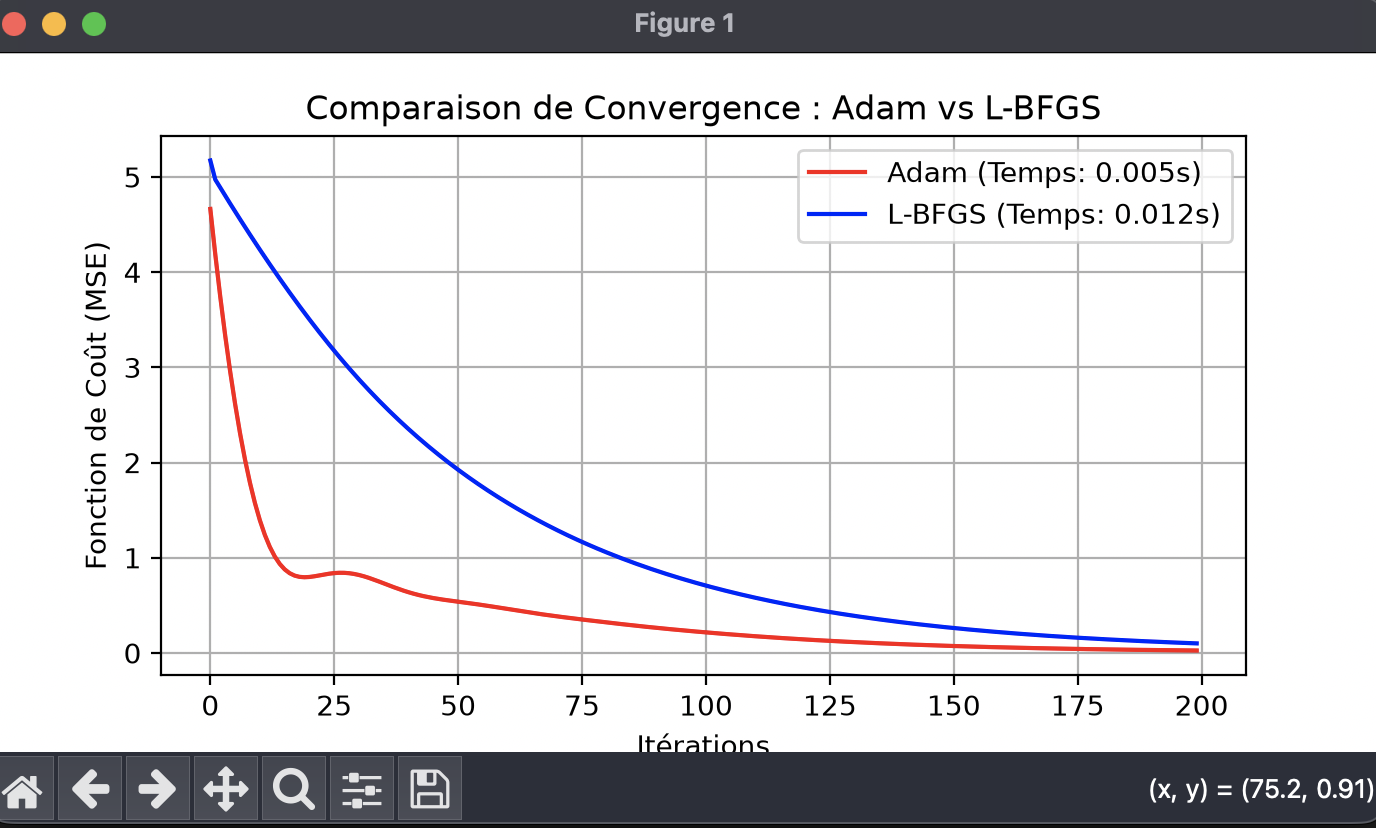
\includegraphics[width=0.75\textheight,keepaspectratio]{image3.png}
    \end{center}
    
    % Note de bas de page analytique basée sur ton graphique
    \footnote{\tiny\textbf{Analyse des résultats \emph{from scratch} :} Sur un problème de régression synthétique de 200 itérations, \textbf{Adam (courbe rouge)} présente une chute de coût agressive et très rapide dès les premières itérations. \textbf{L-BFGS (courbe bleue)} décroît de manière plus linéaire et prudente, le temps d'accumuler assez d'historique de courbure ($s_k, y_k$). Côté performances, notre implémentation montre un avantage en vitesse brute pour Adam ($0.005\text{s}$ contre $0.012\text{s}$), illustrant le surcoût de la récursion à deux boucles en Python pur.}
\end{frame}
\begin{frame}{Références Bibliographiques}
    \begin{thebibliography}{9}
        \bibitem{kingma2014adam} 
        D. P. Kingma, J. Ba, 
        \emph{Adam: A Method for Stochastic Optimization}, 
        ICLR 2015.
        
        \bibitem{gramfort_quasi_newton} 
        A. Gramfort, 
        \emph{Cours de Mathématiques Big Data : (Quasi-)Newton Methods}, 
        Support de cours académique.
        
        \bibitem{synapsara_video} 
        Synapsara, 
        \emph{Optimization Methods Series : BFGS \& L-BFGS}, 
        Capsule vidéo éducative.
        
        \bibitem{sun2019deep}
        J. Sun, Z. Niu, K. A. Inanen, D. Trad,
        \emph{A deep learning perspective of the forward and inverse problems in exploration geophysics},
        Conference Paper, April 2019.
        
        \bibitem{optimizer_history_2020}
        ResearchGate Publication Figures,
        \emph{Optimizing the optimizer for data driven deep neural networks and physics informed neural networks},
        2020.
        
    \end{thebibliography}
\end{frame}

\end{document}